\documentclass[11pt,fleqn, oneside,openany]{book} % Default font size and left-justified equations

% use this list: https://www.educative.io/blog/google-coding-interview

%%%%%%%%%%%%%%%%%%%%%%%%%%%%%%%%%%%%%%%%%%%%
%               Structure
%%%%%%%%%%%%%%%%%%%%%%%%%%%%%%%%%%%%%%%%%%%%
%%%%%%%%%%%%%%%%%%%%%%%%%%%%%%%%%%%%%%%%%
% The Legrand Orange Book
% Structural Definitions File
% Version 2.0 (9/2/15)
%
% Original author:
% Mathias Legrand (legrand.mathias@gmail.com) with modifications by:
% Vel (vel@latextemplates.com)
% 
% This file has been downloaded from:
% http://www.LaTeXTemplates.com
%
% License:
% CC BY-NC-SA 3.0 (http://creativecommons.org/licenses/by-nc-sa/3.0/)
%
%%%%%%%%%%%%%%%%%%%%%%%%%%%%%%%%%%%%%%%%%

%----------------------------------------------------------------------------------------
%	VARIOUS REQUIRED PACKAGES AND CONFIGURATIONS
%----------------------------------------------------------------------------------------

\usepackage[top=3cm,bottom=3cm,left=3cm,right=3cm,headsep=10pt,a4paper]{geometry} % Page margins

\usepackage{graphicx} % Required for including pictures
\graphicspath{{images/}} % Specifies the directory where pictures are stored

\usepackage{lipsum} % Inserts dummy text

\usepackage{tikz} % Required for drawing custom shapes

\usepackage[english]{babel} % English language/hyphenation

\usepackage{enumitem} % Customize lists
\setlist{nolistsep} % Reduce spacing between bullet points and numbered lists

\usepackage{booktabs} % Required for nicer horizontal rules in tables

\usepackage{xcolor} % Required for specifying colors by name
\definecolor{ocre}{RGB}{243,102,25} % Define the orange color used for highlighting throughout the book

%----------------------------------------------------------------------------------------
%	FONTS
%----------------------------------------------------------------------------------------

\usepackage{avant} % Use the Avantgarde font for headings
%\usepackage{times} % Use the Times font for headings
\usepackage{mathptmx} % Use the Adobe Times Roman as the default text font together with math symbols from the Sym­bol, Chancery and Com­puter Modern fonts

\usepackage{microtype} % Slightly tweak font spacing for aesthetics
\usepackage[utf8]{inputenc} % Required for including letters with accents
\usepackage[T1]{fontenc} % Use 8-bit encoding that has 256 glyphs

%----------------------------------------------------------------------------------------
%	BIBLIOGRAPHY AND INDEX
%----------------------------------------------------------------------------------------

\usepackage[citestyle=numeric,sorting=nyt,sortcites=true,autopunct=true,babel=hyphen,hyperref=true,abbreviate=false,backref=true,backend=biber]{biblatex}
\addbibresource{sources/bibliography.bib}
\defbibheading{bibempty}{}

\usepackage{calc} % For simpler calculation - used for spacing the index letter headings correctly
\usepackage{makeidx} % Required to make an index
\makeindex % Tells LaTeX to create the files required for indexing

%----------------------------------------------------------------------------------------
%	MAIN TABLE OF CONTENTS
%----------------------------------------------------------------------------------------

\usepackage{titletoc} % Required for manipulating the table of contents

\contentsmargin{0cm} % Removes the default margin

% Part text styling
\titlecontents{part}[0cm]
{\addvspace{20pt}\centering\large\bfseries}
{}
{}
{}

% Chapter text styling
\titlecontents{chapter}[1.25cm] % Indentation
{\addvspace{12pt}\large\sffamily\bfseries} % Spacing and font options for chapters
{\color{ocre!60}\contentslabel[\Large\thecontentslabel]{1.25cm}\color{ocre}} % Chapter number
{\color{ocre}}  
{\color{ocre!60}\normalsize\;\titlerule*[.5pc]{.}\;\thecontentspage} % Page number

% Section text styling
\titlecontents{section}[1.25cm] % Indentation
{\addvspace{3pt}\sffamily\bfseries} % Spacing and font options for sections
{\contentslabel[\thecontentslabel]{1.25cm}} % Section number
{}
{\hfill\color{black}\thecontentspage} % Page number
[]

% Subsection text styling
\titlecontents{subsection}[1.25cm] % Indentation
{\addvspace{1pt}\sffamily\small} % Spacing and font options for subsections
{\contentslabel[\thecontentslabel]{1.25cm}} % Subsection number
{}
{\ \titlerule*[.5pc]{.}\;\thecontentspage} % Page number
[]

% List of figures
\titlecontents{figure}[0em]
{\addvspace{-5pt}\sffamily}
{\thecontentslabel\hspace*{1em}}
{}
{\ \titlerule*[.5pc]{.}\;\thecontentspage}
[]

% List of tables
\titlecontents{table}[0em]
{\addvspace{-5pt}\sffamily}
{\thecontentslabel\hspace*{1em}}
{}
{\ \titlerule*[.5pc]{.}\;\thecontentspage}
[]

%----------------------------------------------------------------------------------------
%	MINI TABLE OF CONTENTS IN PART HEADS
%----------------------------------------------------------------------------------------

% Chapter text styling
\titlecontents{lchapter}[0em] % Indenting
{\addvspace{15pt}\large\sffamily\bfseries} % Spacing and font options for chapters
{\color{ocre}\contentslabel[\Large\thecontentslabel]{1.25cm}\color{ocre}} % Chapter number
{}  
{\color{ocre}\normalsize\sffamily\bfseries\;\titlerule*[.5pc]{.}\;\thecontentspage} % Page number

% Section text styling
\titlecontents{lsection}[0em] % Indenting
{\sffamily\small} % Spacing and font options for sections
{\contentslabel[\thecontentslabel]{1.25cm}} % Section number
{}
{}

% Subsection text styling
\titlecontents{lsubsection}[.5em] % Indentation
{\normalfont\footnotesize\sffamily} % Font settings
{}
{}
{}

%----------------------------------------------------------------------------------------
%	PAGE HEADERS
%----------------------------------------------------------------------------------------

\usepackage{fancyhdr} % Required for header and footer configuration

\pagestyle{fancy}
\renewcommand{\chaptermark}[1]{\markboth{\sffamily\normalsize\bfseries\chaptername\ \thechapter.\ #1}{}} % Chapter text font settings
\renewcommand{\sectionmark}[1]{\markright{\sffamily\normalsize\thesection\hspace{5pt}#1}{}} % Section text font settings
\fancyhf{} \fancyhead[LE,RO]{\sffamily\normalsize\thepage} % Font setting for the page number in the header
\fancyhead[LO]{\rightmark} % Print the nearest section name on the left side of odd pages
\fancyhead[RE]{\leftmark} % Print the current chapter name on the right side of even pages
\renewcommand{\headrulewidth}{0.5pt} % Width of the rule under the header
\addtolength{\headheight}{2.5pt} % Increase the spacing around the header slightly
\renewcommand{\footrulewidth}{0pt} % Removes the rule in the footer
\fancypagestyle{plain}{\fancyhead{}\renewcommand{\headrulewidth}{0pt}} % Style for when a plain pagestyle is specified

% Removes the header from odd empty pages at the end of chapters
\makeatletter
\renewcommand{\cleardoublepage}{
\clearpage\ifodd\c@page\else
\hbox{}
\vspace*{\fill}
\thispagestyle{empty}
\newpage
\fi}

%----------------------------------------------------------------------------------------
%	THEOREM STYLES
%----------------------------------------------------------------------------------------


\usepackage{amsmath,amsfonts,amssymb,amsthm,mathtools} % For math equations, theorems, symbols, etc
\DeclarePairedDelimiter\ceil{\lceil}{\rceil}
\DeclarePairedDelimiter\floor{\lfloor}{\rfloor}

\newcommand{\intoo}[2]{\mathopen{]}#1\,;#2\mathclose{[}}
\newcommand{\ud}{\mathop{\mathrm{{}d}}\mathopen{}}
\newcommand{\intff}[2]{\mathopen{[}#1\,;#2\mathclose{]}}
\newtheorem{notation}{Notation}[chapter]

% Boxed/framed environments
\newtheoremstyle{ocrenumbox}% % Theorem style name
{0pt}% Space above
{0pt}% Space below
{\normalfont}% % Body font
{}% Indent amount
{\small\bf\sffamily\color{ocre}}% % Theorem head font
{\;}% Punctuation after theorem head
{0.25em}% Space after theorem head
{\small\sffamily\color{ocre}\thmname{#1}\nobreakspace\thmnumber{\@ifnotempty{#1}{}\@upn{#2}}% Theorem text (e.g. Theorem 2.1)
\thmnote{\nobreakspace\the\thm@notefont\sffamily\bfseries\color{black}---\nobreakspace#3.}} % Optional theorem note
\renewcommand{\qedsymbol}{$\blacksquare$}% Optional qed square

\newtheoremstyle{blacknumex}% Theorem style name
{5pt}% Space above
{5pt}% Space below
{\normalfont}% Body font
{} % Indent amount
{\small\bf\sffamily}% Theorem head font
{\;}% Punctuation after theorem head
{0.25em}% Space after theorem head
{\small\sffamily{\tiny\ensuremath{\blacksquare}}\nobreakspace\thmname{#1}\nobreakspace\thmnumber{\@ifnotempty{#1}{}\@upn{#2}}% Theorem text (e.g. Theorem 2.1)
\thmnote{\nobreakspace\the\thm@notefont\sffamily\bfseries---\nobreakspace#3.}}% Optional theorem note

\newtheoremstyle{blacknumbox} % Theorem style name
{0pt}% Space above
{0pt}% Space below
{\normalfont}% Body font
{}% Indent amount
{\small\bf\sffamily}% Theorem head font
{\;}% Punctuation after theorem head
{0.25em}% Space after theorem head
{\small\sffamily\thmname{#1}\nobreakspace\thmnumber{\@ifnotempty{#1}{}\@upn{#2}}% Theorem text (e.g. Theorem 2.1)
\thmnote{\nobreakspace\the\thm@notefont\sffamily\bfseries---\nobreakspace#3.}}% Optional theorem note

% Non-boxed/non-framed environments
\newtheoremstyle{ocrenum}% % Theorem style name
{5pt}% Space above
{5pt}% Space below
{\normalfont}% % Body font
{}% Indent amount
{\small\bf\sffamily\color{ocre}}% % Theorem head font
{\;}% Punctuation after theorem head
{0.25em}% Space after theorem head
{\small\sffamily\color{ocre}\thmname{#1}\nobreakspace\thmnumber{\@ifnotempty{#1}{}\@upn{#2}}% Theorem text (e.g. Theorem 2.1)
\thmnote{\nobreakspace\the\thm@notefont\sffamily\bfseries\color{black}---\nobreakspace#3.}} % Optional theorem note
\renewcommand{\qedsymbol}{$\blacksquare$}% Optional qed square
\makeatother

% Defines the theorem text style for each type of theorem to one of the three styles above
\newcounter{dummy} 
\numberwithin{dummy}{section}
\theoremstyle{ocrenumbox}
\newtheorem{theoremeT}[dummy]{Theorem}

\newtheorem{problem}{Exercise}[chapter]
\newtheorem{exerciseT}{Problem}
\theoremstyle{blacknumex}
\newtheorem{solution}{Solution}[chapter]
\newtheorem{solutionT}{solution}[chapter]
\theoremstyle{blacknumex}
\newtheorem{exampleT}{Example}[chapter]
\theoremstyle{blacknumbox}
\newtheorem{vocabulary}{Vocabulary}[chapter]
\newtheorem{definitionT}{Definition}[section]
\newtheorem{corollaryT}[dummy]{Corollary}
\theoremstyle{ocrenum}
\newtheorem{proposition}[dummy]{Proposition}

%----------------------------------------------------------------------------------------
%	DEFINITION OF COLORED BOXES
%----------------------------------------------------------------------------------------

\RequirePackage[framemethod=default]{mdframed} % Required for creating the theorem, definition, exercise and corollary boxes

% Theorem box
\newmdenv[skipabove=7pt,
skipbelow=7pt,
backgroundcolor=black!5,
linecolor=ocre,
innerleftmargin=5pt,
innerrightmargin=5pt,
innertopmargin=5pt,
leftmargin=0cm,
rightmargin=0cm,
innerbottommargin=5pt]{tBox}

% Exercise box	  
\newmdenv[skipabove=7pt,
skipbelow=7pt,
rightline=false,
leftline=true,
topline=false,
bottomline=false,
backgroundcolor=ocre!10,
linecolor=ocre,
innerleftmargin=5pt,
innerrightmargin=5pt,
innertopmargin=5pt,
innerbottommargin=5pt,
leftmargin=0cm,
rightmargin=0cm,
linewidth=4pt]{eBox}	

% Definition box
\newmdenv[skipabove=7pt,
skipbelow=7pt,
rightline=false,
leftline=true,
topline=false,
bottomline=false,
linecolor=ocre,
innerleftmargin=5pt,
innerrightmargin=5pt,
innertopmargin=0pt,
leftmargin=0cm,
rightmargin=0cm,
linewidth=4pt,
innerbottommargin=0pt]{dBox}	

% Corollary box
\newmdenv[skipabove=7pt,
skipbelow=7pt,
rightline=false,
leftline=true,
topline=false,
bottomline=false,
linecolor=gray,
backgroundcolor=black!5,
innerleftmargin=5pt,
innerrightmargin=5pt,
innertopmargin=5pt,
leftmargin=0cm,
rightmargin=0cm,
linewidth=4pt,
innerbottommargin=5pt]{cBox}

% Creates an environment for each type of theorem and assigns it a theorem text style from the "Theorem Styles" section above and a colored box from above
\newenvironment{theorem}{\begin{tBox}\begin{theoremeT}}{\end{theoremeT}\end{tBox}}
\newenvironment{exercise}{\begin{eBox}\begin{exerciseT}}{\hfill{\color{ocre}\tiny\ensuremath{\blacksquare}}\end{exerciseT}\end{eBox}}				  
\newenvironment{definition}{\begin{dBox}\begin{definitionT}}{\end{definitionT}\end{dBox}}	
\newenvironment{example}{\begin{exampleT}}{\hfill{\tiny\ensuremath{\blacksquare}}\end{exampleT}}		
\newenvironment{corollary}{\begin{cBox}\begin{corollaryT}}{\end{corollaryT}\end{cBox}}	

%----------------------------------------------------------------------------------------
%	REMARK ENVIRONMENT
%----------------------------------------------------------------------------------------

\newenvironment{remark}{\par\vspace{10pt}\small % Vertical white space above the remark and smaller font size
\begin{list}{}{
\leftmargin=35pt % Indentation on the left
\rightmargin=25pt}\item\ignorespaces % Indentation on the right
\makebox[-2.5pt]{\begin{tikzpicture}[overlay]
\node[draw=ocre!60,line width=1pt,circle,fill=ocre!25,font=\sffamily\bfseries,inner sep=2pt,outer sep=0pt] at (-15pt,0pt){\textcolor{ocre}{R}};\end{tikzpicture}} % Orange R in a circle
\advance\baselineskip -1pt}{\end{list}\vskip5pt} % Tighter line spacing and white space after remark

%----------------------------------------------------------------------------------------
%	SECTION NUMBERING IN THE MARGIN
%----------------------------------------------------------------------------------------

\makeatletter
\renewcommand{\@seccntformat}[1]{\llap{\textcolor{ocre}{\csname the#1\endcsname}\hspace{1em}}}                    
\renewcommand{\section}{\@startsection{section}{1}{\z@}
{-4ex \@plus -1ex \@minus -.4ex}
{1ex \@plus.2ex }
{\normalfont\large\sffamily\bfseries}}
\renewcommand{\subsection}{\@startsection {subsection}{2}{\z@}
{-3ex \@plus -0.1ex \@minus -.4ex}
{0.5ex \@plus.2ex }
{\normalfont\sffamily\bfseries}}
\renewcommand{\subsubsection}{\@startsection {subsubsection}{3}{\z@}
{-2ex \@plus -0.1ex \@minus -.2ex}
{.2ex \@plus.2ex }
{\normalfont\small\sffamily\bfseries}}                        
\renewcommand\paragraph{\@startsection{paragraph}{4}{\z@}
{-2ex \@plus-.2ex \@minus .2ex}
{.1ex}
{\normalfont\small\sffamily\bfseries}}

%----------------------------------------------------------------------------------------
%	PART HEADINGS
%----------------------------------------------------------------------------------------

% numbered part in the table of contents
\newcommand{\@mypartnumtocformat}[2]{%
\setlength\fboxsep{0pt}%
\noindent\colorbox{ocre!20}{\strut\parbox[c][.7cm]{\ecart}{\color{ocre!70}\Large\sffamily\bfseries\centering#1}}\hskip\esp\colorbox{ocre!40}{\strut\parbox[c][.7cm]{\linewidth-\ecart-\esp}{\Large\sffamily\centering#2}}}%
%%%%%%%%%%%%%%%%%%%%%%%%%%%%%%%%%%
% unnumbered part in the table of contents
\newcommand{\@myparttocformat}[1]{%
\setlength\fboxsep{0pt}%
\noindent\colorbox{ocre!40}{\strut\parbox[c][.7cm]{\linewidth}{\Large\sffamily\centering#1}}}%
%%%%%%%%%%%%%%%%%%%%%%%%%%%%%%%%%%
\newlength\esp
\setlength\esp{4pt}
\newlength\ecart
\setlength\ecart{1.2cm-\esp}
\newcommand{\thepartimage}{}%
\newcommand{\partimage}[1]{\renewcommand{\thepartimage}{#1}}%
\def\@part[#1]#2{%
\ifnum \c@secnumdepth >-2\relax%
\refstepcounter{part}%
\addcontentsline{toc}{part}{\texorpdfstring{\protect\@mypartnumtocformat{\thepart}{#1}}{\partname~\thepart\ ---\ #1}}
\else%
\addcontentsline{toc}{part}{\texorpdfstring{\protect\@myparttocformat{#1}}{#1}}%
\fi%
\startcontents%
\markboth{}{}%
{\thispagestyle{empty}%
\begin{tikzpicture}[remember picture,overlay]%
\node at (current page.north west){\begin{tikzpicture}[remember picture,overlay]%	
\fill[ocre!20](0cm,0cm) rectangle (\paperwidth,-\paperheight);
\node[anchor=north] at (4cm,-3.25cm){\color{ocre!40}\fontsize{220}{100}\sffamily\bfseries\@Roman\c@part}; 
\node[anchor=south east] at (\paperwidth-1cm,-\paperheight+1cm){\parbox[t][][t]{8.5cm}{
\printcontents{l}{0}{\setcounter{tocdepth}{1}}%
}};
\node[anchor=north east] at (\paperwidth-1.5cm,-3.25cm){\parbox[t][][t]{15cm}{\strut\raggedleft\color{white}\fontsize{30}{30}\sffamily\bfseries#2}};
\end{tikzpicture}};
\end{tikzpicture}}%
\@endpart}
\def\@spart#1{%
\startcontents%
\phantomsection
{\thispagestyle{empty}%
\begin{tikzpicture}[remember picture,overlay]%
\node at (current page.north west){\begin{tikzpicture}[remember picture,overlay]%	
\fill[ocre!20](0cm,0cm) rectangle (\paperwidth,-\paperheight);
\node[anchor=north east] at (\paperwidth-1.5cm,-3.25cm){\parbox[t][][t]{15cm}{\strut\raggedleft\color{white}\fontsize{30}{30}\sffamily\bfseries#1}};
\end{tikzpicture}};
\end{tikzpicture}}
\addcontentsline{toc}{part}{\texorpdfstring{%
\setlength\fboxsep{0pt}%
\noindent\protect\colorbox{ocre!40}{\strut\protect\parbox[c][.7cm]{\linewidth}{\Large\sffamily\protect\centering #1\quad\mbox{}}}}{#1}}%
\@endpart}
\def\@endpart{\vfil\newpage
\if@twoside
\if@openright
\null
\thispagestyle{empty}%
\newpage
\fi
\fi
\if@tempswa
\twocolumn
\fi}

%----------------------------------------------------------------------------------------
%	CHAPTER HEADINGS
%----------------------------------------------------------------------------------------

% A switch to conditionally include a picture, implemented by  Christian Hupfer
\newif\ifusechapterimage
\usechapterimagetrue
\newcommand{\thechapterimage}{}%
\newcommand{\chapterimage}[1]{\ifusechapterimage\renewcommand{\thechapterimage}{#1}\fi}%
\def\@makechapterhead#1{%
{\parindent \z@ \raggedright \normalfont
\ifnum \c@secnumdepth >\m@ne
\if@mainmatter
\begin{tikzpicture}[remember picture,overlay]
\node at (current page.north west)
{\begin{tikzpicture}[remember picture,overlay]
\node[anchor=north west,inner sep=0pt] at (0,0) {\ifusechapterimage\includegraphics[width=\paperwidth]{\thechapterimage}\fi};
\draw[anchor=west] (\Gm@lmargin,-4cm) node [line width=2pt,rounded corners=15pt,draw=ocre,fill=white,fill opacity=0.5,inner sep=15pt]{\strut\makebox[22cm]{}};
\draw[anchor=west] (\Gm@lmargin+.3cm,-4cm) node {\huge\sffamily\bfseries\color{black}\thechapter. #1\strut};
\end{tikzpicture}};
\end{tikzpicture}
\else
\begin{tikzpicture}[remember picture,overlay]
\node at (current page.north west)
{\begin{tikzpicture}[remember picture,overlay]
\node[anchor=north west,inner sep=0pt] at (0,0) {\ifusechapterimage\includegraphics[width=\paperwidth]{\thechapterimage}\fi};
\draw[anchor=west] (\Gm@lmargin,-4cm) node [line width=2pt,rounded corners=15pt,draw=ocre,fill=white,fill opacity=0.5,inner sep=15pt]{\strut\makebox[22cm]{}};
\draw[anchor=west] (\Gm@lmargin+.3cm,-4cm) node {\huge\sffamily\bfseries\color{black}#1\strut};
\end{tikzpicture}};
\end{tikzpicture}
\fi\fi\par\vspace*{100\p@}}}

%-------------------------------------------

\def\@makeschapterhead#1{%
\begin{tikzpicture}[remember picture,overlay]
\node at (current page.north west)
{\begin{tikzpicture}[remember picture,overlay]
\node[anchor=north west,inner sep=0pt] at (0,0) {\ifusechapterimage\includegraphics[width=\paperwidth]{\thechapterimage}\fi};
\draw[anchor=west] (\Gm@lmargin,-4cm) node [line width=2pt,rounded corners=15pt,draw=ocre,fill=white,fill opacity=0.5,inner sep=15pt]{\strut\makebox[22cm]{}};
\draw[anchor=west] (\Gm@lmargin+.3cm,-4cm) node {\huge\sffamily\bfseries\color{black}#1\strut};
\end{tikzpicture}};
\end{tikzpicture}
\par\vspace*{100\p@}}
\makeatother

%----------------------------------------------------------------------------------------
%	HYPERLINKS IN THE DOCUMENTS
%----------------------------------------------------------------------------------------

\usepackage{hyperref}
\hypersetup{hidelinks,backref=true,pagebackref=true,hyperindex=true,colorlinks=false,breaklinks=true,urlcolor= ocre,bookmarks=true,bookmarksopen=false,pdftitle={Title},pdfauthor={Author}}
\usepackage{bookmark}
\bookmarksetup{
open,
numbered,
addtohook={%
\ifnum\bookmarkget{level}=0 % chapter
\bookmarksetup{bold}%
\fi
\ifnum\bookmarkget{level}=-1 % part
\bookmarksetup{color=ocre,bold}%
\fi
}
}

%----------------------------------------------------------------------------------------
%	LISTINGS
%----------------------------------------------------------------------------------------
%----------------------------------------------------------------------------------------
%	LISTINGS
%----------------------------------------------------------------------------------------
\usepackage{listings}
\lstset{language=C++}
\lstset{
	basicstyle=\footnotesize\ttfamily,
	breaklines=true,
	showstringspaces=false,
	numbers=left,
	backgroundcolor=\color{bgcolor},
	commentstyle=\color{gray},
	keywordstyle=\color{blue},
	keywordstyle=[2]\color{teal},   % cyan or teal can also be a good choice, use \bfseries for bold
	frame=none,                     % adds a frame around the code
	tabsize=2,                      % sets default tabsize to 2 spaces
	captionpos=b,                   % sets the caption-position to bottom
	morekeywords=[2]{}              % if you want to add more keywords to the set
	__
}

\definecolor{mygreen}{RGB}{28,172,0} % color values Red, Green, Blue
\definecolor{mylilas}{RGB}{170,55,241}
\lstset{language=Matlab,%
    %basicstyle=\color{red},
    breaklines=true,%
    morekeywords={matlab2tikz},
    keywordstyle=\color{blue},%
    morekeywords=[2]{1}, keywordstyle=[2]{\color{black}},
    identifierstyle=\color{black},%
    stringstyle=\color{mylilas},
    commentstyle=\color{mygreen},%
    showstringspaces=false,%without this there will be a symbol in the places where there is a space
    numbers=left,%
    numberstyle={\tiny \color{black}},% size of the numbers
    numbersep=9pt, % this defines how far the numbers are from the text
    emph=[1]{for,end,break},emphstyle=[1]\color{red}, %some words to emphasise
    %emph=[2]{word1,word2}, emphstyle=[2]{style},    
}

\usepackage{color}
\definecolor{bgcolor}{rgb}{0.98,0.98,0.98}


%----------------------------------------------------------------------------------------

%	QandA

%----------------------------------------------------------------------------------------

\newenvironment{QandA}{\begin{enumerate}[label=\bfseries Q.\arabic*.,leftmargin=2em,rightmargin=2em]\bfseries}{\end{enumerate}}
\newenvironment{answered}{\par\normalfont}{}
%----------------------------------------------------------------------------------------
%	ALGORITHM
%----------------------------------------------------------------------------------------
\usepackage[]{algorithm2e}

\RestyleAlgo{boxruled}
\usepackage{mdframed,framed}

\SetKwProg{Fn}{Function}{}{}
\SetKwRepeat{Do}{do}{while}%
\SetKwFunction{CreateHashSet}{CreateHashSet<int>}


\DeclarePairedDelimiter\abs{\lvert}{\rvert}%
\DeclarePairedDelimiter\norm{\lVert}{\rVert}%

% Swap the definition of \abs* and \norm*, so that \abs
% and \norm resizes the size of the brackets, and the 
% starred version does not.
\makeatletter
\let\oldabs\abs
\def\abs{\@ifstar{\oldabs}{\oldabs*}}
%
\let\oldnorm\norm
\def\norm{\@ifstar{\oldnorm}{\oldnorm*}}
\makeatother

\usepackage[makeroom]{cancel}


\interfootnotelinepenalty=10000

\begin{document}

%\frontmatter
%\begingroup
%\thispagestyle{empty}
%\begin{tikzpicture}[remember picture,overlay]
%  \coordinate [below=12cm] (midpoint) at (current page.north);
%  \node at (current page.north west)
%  {\begin{tikzpicture}[remember picture,overlay]
%      \node[anchor=north west,inner sep=0pt] at (0,0) {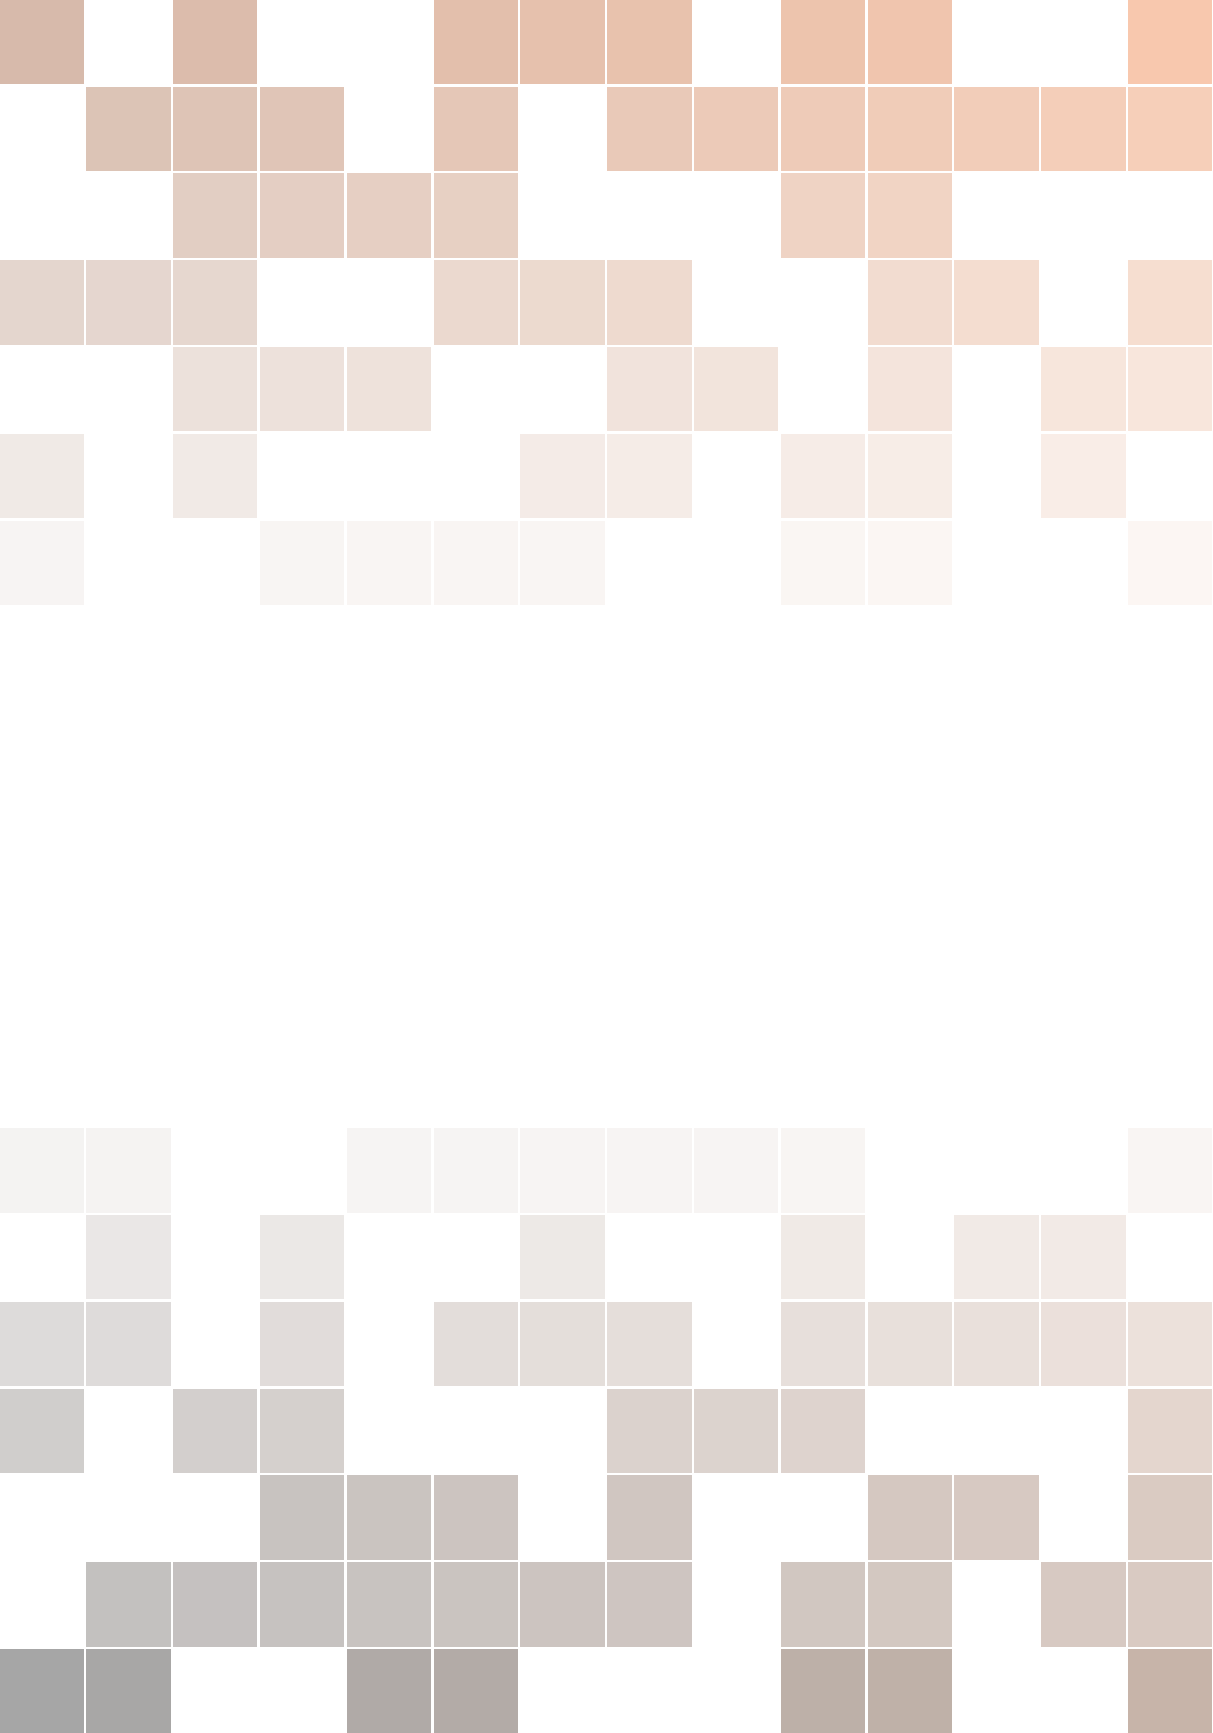
\includegraphics[width=\paperwidth]{images/background}}; % Background image
%\textsl{}
%      \draw[anchor=north] (midpoint) node [fill=ocre!30!white,fill opacity=0.6,text opacity=1,inner sep=1cm]{\Huge\centering\bfseries\sffamily\parbox[c][][t]{\paperwidth}{\centering Coding Interview Essentials\\[15pt] % Book title
%      {\Large - }\\[20pt] % Subtitle
%      {\huge Davide Spataro}}}; % Author name
%    \end{tikzpicture}};
%\end{tikzpicture}
%\vfill
%\endgroup


\includepdf[pages={2},fitpaper=true]{images/book_covers1.pdf}


\usechapterimagefalse % If you don't want to include a chapter image, use this to toggle images off - it can be enabled later with \usechapterimagetrue

%\chapterimage{images/header} % Table of contents heading image

\pagestyle{empty} % No headers

\tableofcontents % Print the table of contents itself

%\lstlistoflistings
%\listoffigures
%\listoftables

%\cleardoublepage % Forces the first chapter to start on an odd page so it's on the right

%pagestyle{fancy} % Print headers again

%!TEX root = ../main.tex
%%%%%%%%%%%%%%%%%%%%%%%%%%%%%%%%%%
% Links:
%
% Difficulty:
% Companies: 
%%%%%%%%%%%%%%%%%%%%%%%%%%%%%%%%%%

\chapter{Coin Change Problem}
\label{ch:coin_change}
\section*{Introduction}
The problem discussed in this chapter is considered by many to be a fundamental stepping stone for anyone on the path towards mastering Dynamic Programming (see Section \ref{sect:appendix:DP}).
This reputation originates from the fact that this problem encompasses all the crucial ingredients of any DP algorithm with the additional benefit of having a very intuitive statement as 
it features things like coins and change that are concepts we are all familiar with.

This problem addresses the question of finding the minimum number of coins that add up to a given amount of money. 
Many people, when reading the statement of this problem, are tempted to approach it greedily but, as we will see, this does not always (despite it actually often does) lead to the correct answer. 

The coin change problem can be seen as an archetype for a whole bunch of DP optimization problems that can be reduced and solved, using the techniques shown in this section (see Chapter \ref{ch:dice_rolls} and \ref{ch:can_jump}, for instance).


\section{Problem statement}
\begin{exercise}
Write a function that, given an array of coin denominations $I$ and an integer $t$ representing an amount of money, returns
the minimum number of coins (of any denomination in $I$) that are necessary obtain $t$. 
You have an infinite amount of coins of each denomination. 

	\begin{example}
		\label{ex:coin_change:example1}
		\hfill \\
		Given $I=\{1,2,5\}$ and $t=11$, the function returns $3$.
		We can change $11$ in many ways, but none of them uses less than $3$ coins:
		\begin{itemize*}
			\item \textbf{two} coins of denomination $5$, and
			\item \textbf{one} coin of denomination $1$.
		\end{itemize*}
	\end{example}

	\begin{example}
		\hfill \\
		Given $I=\{1,3,4,5\}$ and $t=7$, the function returns $2$.
		We can change $7$ by using 
		\begin{itemize*}
			\item \textbf{one} coin of value $3$ and
			\item \textbf{one} of value $4$.
		\end{itemize*}
	\end{example}

	\begin{example}
		\label{ex:coin_change:example3}
		\hfill \\
		Given $I=\{1,5,8\}$ and $t=12$, the function returns $4$.
		We can change $12$ by using
		\begin{itemize*}
			\item \textbf{two} coins of value $1$ and
			\item \textbf{two} of value $5$.
		\end{itemize*}
	\end{example}
\end{exercise}

\section{Clarification Questions}

\begin{QandA}

	\item Can $I$ be empty?
	\begin{answered}
		\textit{Yes.}
	\end{answered}

	\item Is $I$ sorted?
	\begin{answered}
		\textit{No, denominations in $I$ are not sorted.}
	\end{answered}

	\item Can we assume we can always change $t$ using the denomination in $I$?
	\begin{answered}
		\textit{No, and if that is the case the function should return $-1$.}
	\end{answered}
	
\end{QandA}

\section{Discussion}
\label{coin_change:sec:discussion}

\subsection{The greedy approach and why it is incorrect}
This is one of those problems that can trick inexperienced candidates into thinking about a greedy approach, especially when nudged by the examples given along with the statement that are crafted so that a greedy approach produces the optimal answer.

A greedy algorithm for this problem works by repeatedly picking the largest coin $I_k$ that is smaller than $t$, and repeating the process on a new target amount $t-I_k$ until we reach $0$.
Listing \ref{list:coin_change:greedy} shows a possible implementation of this algorithm.

If we apply this algorithm to the Example \ref{ex:coin_change:example1}  we see that initially $t=11$
and that the largest denomination $5$ is smaller that $t$. Therefore we pick it (in the code this is reflected in assigning the variable \inline{greedy_choice = *it}) and we decrease $t$ by the same amount.
Now, $t=6$ which is still larger than $5$. We pick $5$ again and $t = 1$.
At this point neither $5$ nor $2$ are smaller or equal than $1$ and we choose $1$ which is the only denomination that is smaller or equal than the current value of $t$.
Now $t=0$ and we can stop, after having used $3$ coins in total, which is optimal.

However if we try the same algorithm on the Example \ref{ex:coin_change:example3} we get the answer $6$ which is quite far off from the optimum $4$. 
This approach is also not complete as it fails to find a valid solution like in the case where $I=\{2,5,8\}$ and $t=12$. In this case the greedy algorithm returns $-1$, when it is perfectly possible to change the amount $12$ by using 
\begin{itemize*}
	\item \textbf{two} coins of value $5$ and,
	\item \textbf{one} coin of value $2$.
\end{itemize*}	

\lstinputlisting[language=c++, caption={Greedy solution which always try to use the largest coin we can. Notice tht this approach is incorrect and should not be used during an interview.},label=list:coin_change:greedy]{sources/coin_change/coin_change_solution_greedy.cpp}



\subsection{Fomulation as an optimization problem}
\label{coin_change:sec:mathdefinition}
This problem can be formalized as an optimization problem where the solution is a set of number $X=\{x_0,x_1,\ldots, x_{|I|-1}\}$ of size $|I|$ with each $x_j$ representing how many coins of the denomination $I_j$ are used. 
Given this formulation, the answer is simply the minimum of Equation \ref{eq:coin_change:totalsum} subject to Equation \ref{eq:coin_change:totalsum_constraint}.
\begin{subequations}
\begin{equation}
	W(t) = \sum_{j=0}^{|I|-1} X_j
	\label{eq:coin_change:totalsum}
\end{equation}

\begin{equation}
	\sum_{j=0}^{|I|-1} X_j I_j = t
	\label{eq:coin_change:totalsum_constraint}
\end{equation}
\end{subequations}

$W(t)$ (Equation \ref{eq:coin_change:totalsum}) is the total  number of coins used and the constraint $W(t)$ is subject to (Equation \ref{eq:coin_change:totalsum_constraint}) forces their collective value to be exactly equal to the target amount $t$.

\subsection{Brute-force}
\label{coin_change:sec:bruteforce}
The brute-force approach is conceptually straightforward and consists in enumerating and checking every single possible valid combination of coins
while keeping track of the one with the fewest number of coins adding up to $t$.
A valid combination is described by an instance of the  array $X$ mentioned above in Section \ref{coin_change:sec:mathdefinition}.

The enumeration process can be implemented using recursion and backtracking. 
The idea is that we fill $X$ (which initially is zeroed) incrementally, by starting with the first position, $X_0$.
A value in $X$ at position $j$ ($x_j$) represents the number of coins of the denomination $I_j$ (contributing for a total value of $I_j X_j$). 

When we try a new value $k$ for $x_0$, we know we are adding $kI_0$ to the overall value of all the coins in $X$, and of course also that we used $k$ more coins.
Once a decision regarding the number of coins of value $I_0$ we use is made, we can continue and try to fill the next position of $X$ knowing that we have to make up for $t-(kI_0)$ and that we have used already $k$ coins. 

This process can be repeated until either we reach a point where we have nothing to make up for anymore, or we still have some amount left to change but, no available denominations to use.
In the former case we return the number of coins used up to that point (or we compare it to the current minimum so far), while in the latter, we return a value indicating that there is no solution (usually a large number).

An implementation of this idea is shown below in Listing \ref{list:coin_change:bruteforce}.
Notice that the function \inline{change_ways_bruteforce_backtracking_helper} takes $4$ parameters:
\begin{enumerate}
	\item \inline{I}: a read-only parameter containing the denominations;
	\item \inline{t}: the amount we need to make up for;
	\item \inline{j}: the index of the denomination in $I$ we are currently processing;
	\item \inline{coin_used}: the number of coin used so far.
\end{enumerate}


\lstinputlisting[language=c++, caption={Backtracking recursive brute-force solution},label=list:coin_change:bruteforce]{sources/coin_change/coin_change_solution3.cpp}

The function is initially called with $j=0$ (indicating we start with the first denomination), \inline{coin_used = 0} (no coins are used) and \inline{t} is set to be equal to the original amount (the one coming from the main driver function \inline{change_ways_bruteforce}).
As the execution and the recursion unfold, $t$ is changed accordingly to the value of the $k$ coins of denomination $I_j$ we are trying to use, \inline{coin_used} is incremented by $k$, and $j$ is incremented by one.

Figure \ref{fig:coin_change:recursiontree} shows the recursion tree of \inline{change_ways_bruteforce_backtracking_helper} 
when the input is the one shown in Example \ref{ex:coin_change:example1}; As we can see, there are $4$ ways (highlighted in \textcolor{darkgreen}{green}) of changing $4$ by using coin of denominations $\{1,2,3\}$:
\begin{enumerate}
	\item $2+2$ (two coins of value $2$),
	\item $1+3$, (one and three coins of values $1$ and $3$, respectively)
	\item $1+1+2$, (two and one coins of values $1$ and $2$, respectively), and
	\item $1+1+1+1$ ($4$ coins of value $1$).
\end{enumerate}
\begin{figure}
	\centering
	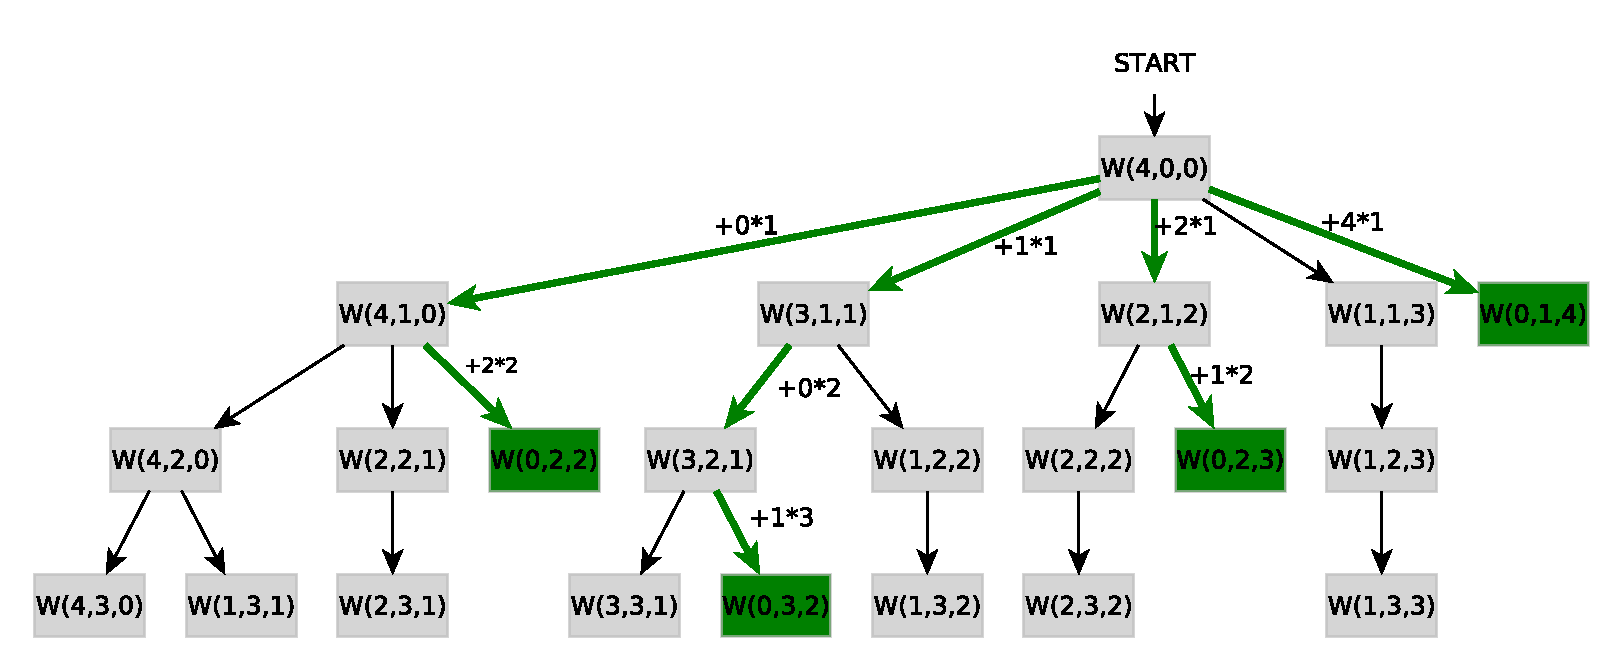
\includegraphics[width=\textwidth]{sources/coin_change/images/recursiontree}
	\captionsetup{singlelinecheck=off}
	\caption{This figure shows the call tree for the recursive function \inline{change_ways_bruteforce_backtracking_helper} on the following input:  $I = \{1,2,3\}$, and $t=4$. Each node contains the only three varying parameters of \inline{change_ways_bruteforce_backtracking_helper} (shortened here as $W$): the first is the current $t$ (the amount that we still need to make up for). The second   is the index to an element of $I$ for the denomination we are considering and the third is the number of coins used so far.
	Moreover, the highlighted paths shows all the valid ways of changing $4$. Note that all the green nodes have the first number equal to zero.}
	\label{fig:coin_change:recursiontree}
\end{figure}

The time complexity of this approach is exponential in $|I|$. 
As an informal proof of this fact consider that for each denomination we at least try either to use zero or one coin. 
Therefore for each element of $I$ we have two choices resulting in $2^{|I|}$ possibilities. 
The space complexity is linear in $|I|$ as in the worst case the depth of the recursive calls do not go deeper than $|I|$. This is a direct consequence of the base case, checking for $j >= |I|$.

\subsection{Dynamic Programming - Top-Down}
\label{sec:coin_change:topdown}
Like all DP problems, one of the first things we need to do, is to try to define the solution to the problem in terms of solutions to sub-problems
\footnote{The concept of sub-problem, in the context of this problem might seem quite fuzzy; You can think of it as a problem exactly equal to the main one except it operates on an input that
is  somehow \textit{"smaller"} and it is therefore easier to solve.
In this specific case it means $t$  is smaller.}.
Once that is in place, we need to make sure that our formulation satisfies the \textit{optimal substructure} property and, crucially, that also requires the solutions to the same sub-problems
more than once (see Appendix \ref{sect:appendix:DP}). 
Only then we are ready to unleash the full power of DP.

Consider the denominations listed in $I=\{I_0 < I_1 < \ldots \}$ and the function $C(x)$ which returns the minimum number of coins necessary to obtain the amount $x$ using $I$. 
We can calculate the value of $C(y)$ where $y > x$ very easily by using Equation \ref{eq:coin_change:dpformula}:
\begin{equation}
	\begin{cases}
		C(0) = 0 \\
		C(y) = +\infty \: \: \text{if} \: \: x < 0 \\
 		C(y) = 1 + \min_{d \in I} C(y-d)
	 \end{cases}
	\label{eq:coin_change:dpformula}
\end{equation}
We can see see that, the answer for the amount $y$ can be expressed in terms of answers to amount strictly smaller than $y$ and in particular, when:
\begin{itemize}
	\item $y=0$, the answer is $0$ as there is only one way of making up for the amount $0$ i.e. using zero coins;
	\item $y<0$ the answer is $+\infty$, signalling it is impossible to obtain a negative amount by only using positive denominations;
	\item in all the other cases, you can calculate the answer by using the answers to sub-problems for smaller amounts that you can obtain by subtracting the current amount with one of the coin denomination in $I$.
\end{itemize} 
The key point here is that $C(y)$, as it is defined in Equation \ref{eq:coin_change:dpformula} satisfies the optimal substructure property.
In-fact we can see that we can obtain the optimal answer to $C(y)$ from the optimal solution to smaller sub-problems. 

Moreover, if we apply Equation \ref{eq:coin_change:dpformula} to the Example \ref{ex:coin_change:example1} we see that solution to sub-problems are required over and over again:
\begin{itemize}
	\item $C(11) = \min(C(10),C(9), C(6))$
	\item $C(10) = \min(C(9),C(8), C(5))$
	\item $C(9) = \min(C(8),C(7), C(4))$
	\item $C(8) = \min(C(7),C(6), C(3))$
	\item $C(7) = \min(C(6),C(5), C(2))$
	\item $\ldots$
\end{itemize}
Figure \ref{fig:coin_change:DPtree} shows the initials layers of the recursion tree for $C(11)$, from which is it clear that the whole work described by the subtree $C(9)$ is done twice: once from  $C(11)$ when using a coin of value $2$ (\textcolor{red}{red} nodes) and a second time from $C(10)$ when using a coin of value $1$ (\textcolor{orange}{orange} nodes).

\begin{figure}
	\centering
	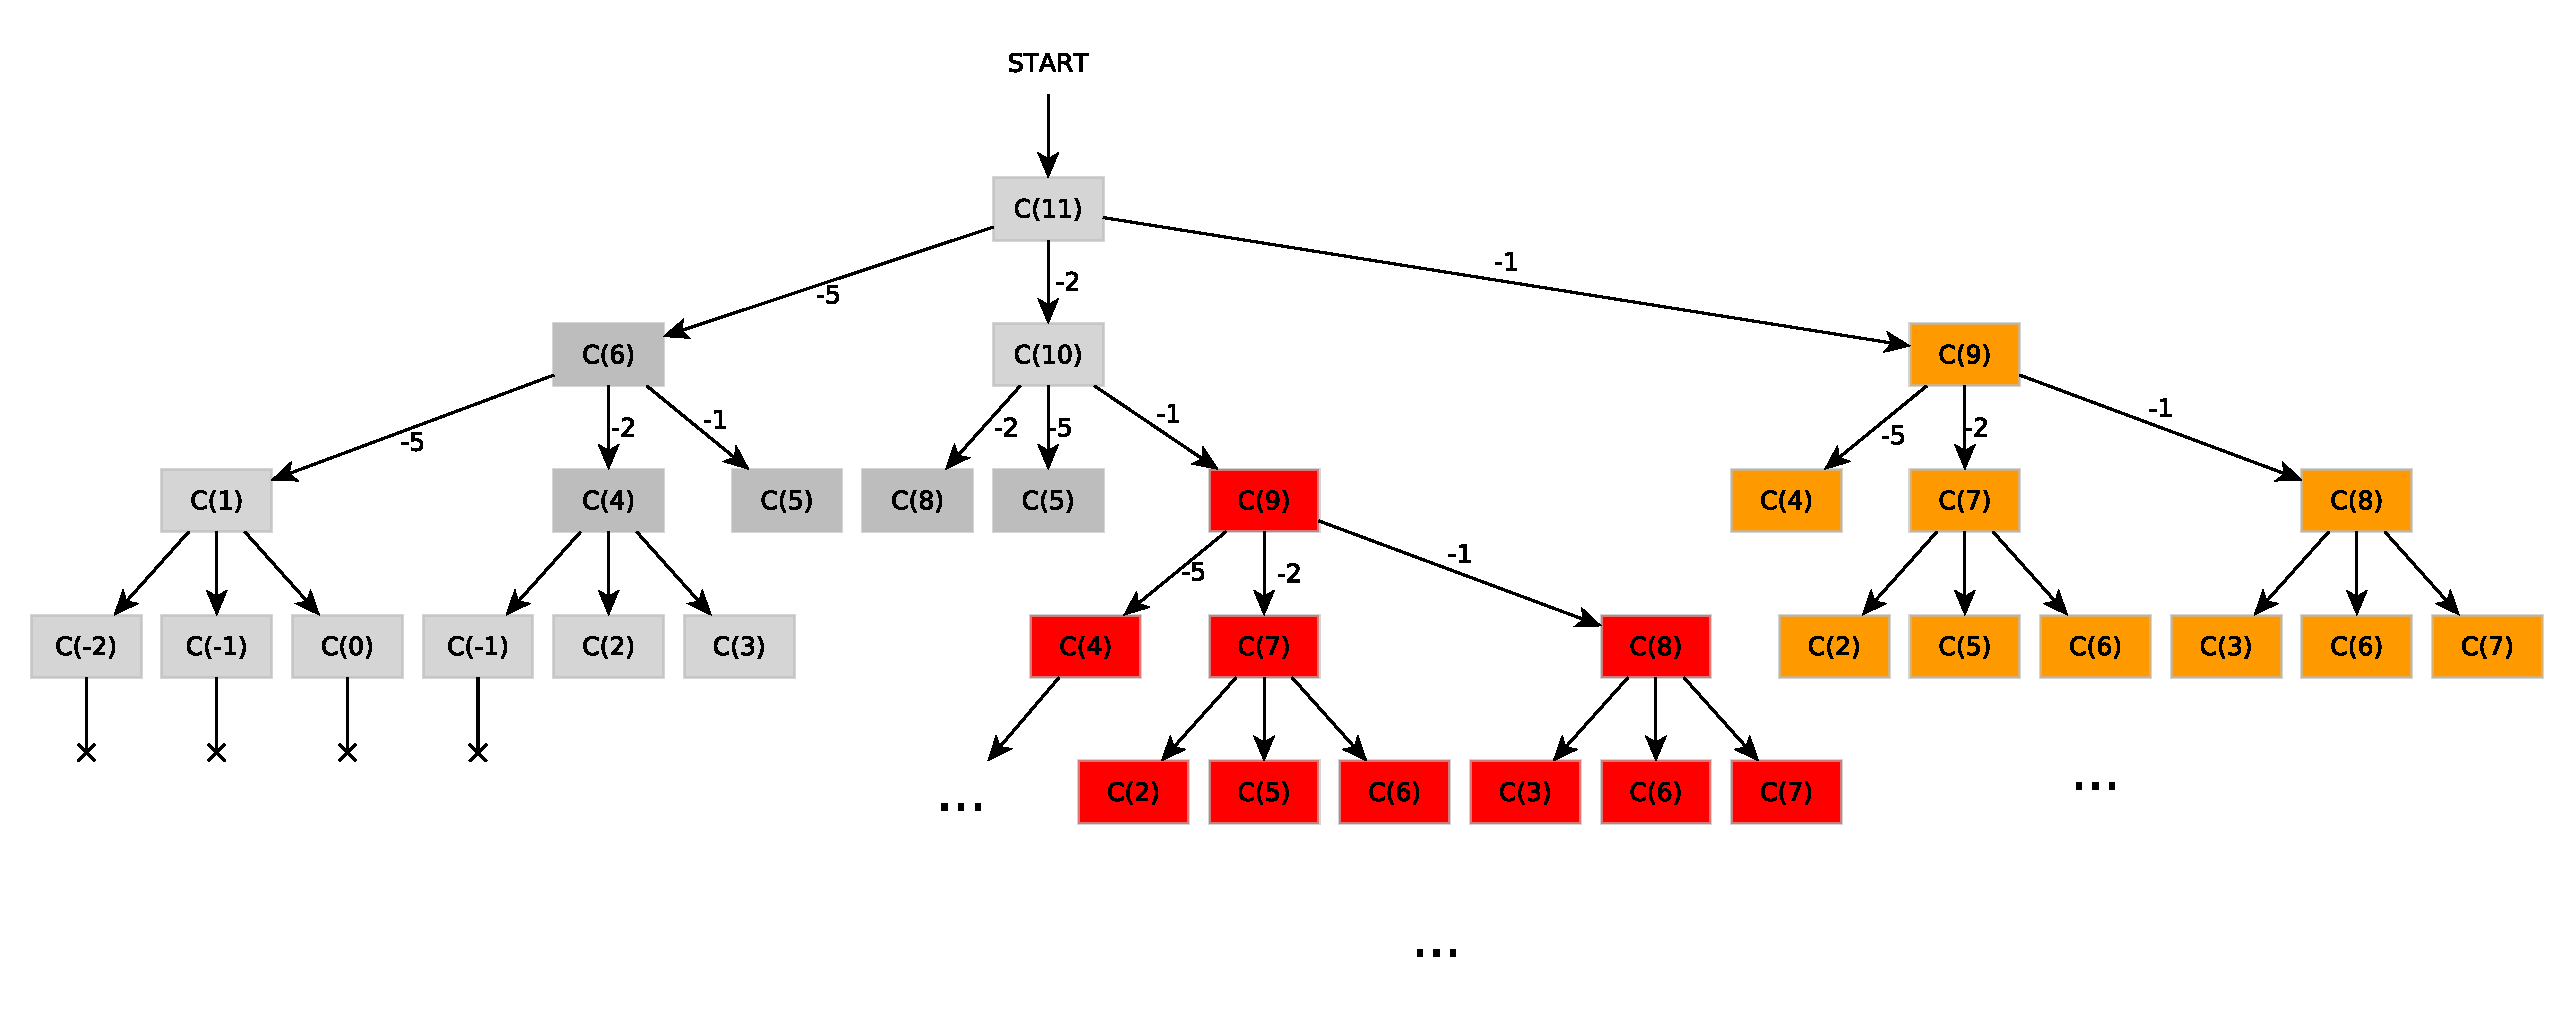
\includegraphics[width=\textwidth]{sources/coin_change/images/DPtree}
	\caption{Initial layers of the recursion tree for $C(11)$}
	\label{fig:coin_change:DPtree}
\end{figure}

Therefore, it seems that this problem also satisfies the overlapping subproblem property and we can very easily turn Equation \ref{eq:coin_change:dpformula} into an efficient DP solution by translating it into a memoized recursive function implementation as shown in Listing \ref{list:coin_change:topdown}.
The code works by blindly following what dictated by Equation \ref{eq:coin_change:dpformula} with the only addition of the function \inline{change_ways_DP_topdown_helper} being memoized via a cache, which takes the shape of a standard \inline{std::unordered_map}.

\lstinputlisting[language=c++, caption={Dynamic Programmin top-down solution.},label=list:coin_change:topdown]{sources/coin_change/coin_change_solution4.cpp}

The time complexity of Listing \ref{list:coin_change:topdown} is $\Theta(t|I|)$: There are $t+1$ possible  distinct calls to \inline{change_ways_DP_topdown_helper} and each of them costs 
$\Theta(|I|)$. The space complexity is $O(t)$ (if you consider the additional space occupied the  by the stack during the recursive process, otherwise it is constant); if $1 \in I$ then we get calls to \inline{change_ways_DP_topdown_helper} for every value from $t$ to $0$.

\subsection{Bottom-up}
\label{coin_change:sec:bottomup}
In Section \ref{sec:coin_change:topdown} we have seen how it is possible to use DP to attach and solve this problem efficiently by adopting a top-down approach. All DP solutions can be also implemented in a bottom-up fashion where we explicitly fill in a DP table ($T$) starting with the known values, usually corresponding to the base cases of the recursion for the top-down formulation.

Let's start by isolating the values of $t$ for which the solution is known. 
A good starting point seems to be the base cases of Listing \ref{list:coin_change:topdown} where $t=0$ and we return $0$ immediately. The next question we want to ask ourselves is, how can we fill cells of the DP table corresponding to higher values of $t$ starting from the value for the cell at $t=0$? The key idea here is that from a given $t$ we can obtain all the amounts corresponding to: $t+I_0,t+I_1,\ldots,  $ with a number of coins equal to the number of coins you needed to obtain $t$ plus $1$.

For instance if $I=\{1,2,5\}$ the DP table $T$ initially is as follows: $T=\{0,+\infty,+\infty,\ldots\}$.
From the value $0$ we can update cells for $t=1,2,5$ with the value $1$ and the the table becomes: $T=\{0,1,1,+\infty,+\infty,1,+\infty,\ldots\}$.
We can now repeat the process from $t=1$ and update all the values you can achieve from $t=1$ i.e. $2,3,6$. 
Notice that we can skip values $2$ and $3$  because they have already been obtained from the amount $1$ with fewer coins. 
$T$ is now: $T=\{0,1,1,2,+\infty,1,1,+\infty,\ldots\}$.
This process can continue until we have finished processing all the values up to $t$ and the final answer will be stored in the DP table cell for the amount $t$. 

More generally, assuming the table is filled up to (and including) cell at index $x+1$ (corresponding to the amount $x$)
you can update the cell of $T$ at index $0 \leq k < |I|$ as follows: $$T_{x+I_k} = \min (T_{x+I_k}, T_{x}+1)$$. 

Listing \ref{list:coin_change:bottomup} shows an implmentation of this idea. The time and space complexities are both $O(|I|\times t)$. 


\lstinputlisting[language=c++, caption={Dynamic Programmin bottom-up solution.},label=list:coin_change:bottomup]{sources/coin_change/coin_change_solution5.cpp}

\subsection{Conclusion}
In this chapter we have seen how to solve the Coin change problem which is a classical DP problem. 

The nice thing about this approach is that, we can reuse it virtually for any DP problem, provided we came up with a suitable recursive definition for the solutions to the subproblem.  All it is necessary is to code such a definition into a recursive function and use memoization to save precious computation steps. You can see more examples of problems solved with a similar techniques in Sections \ref{sect:appendix:DP},\ref{dice_rolls:sec:DP}, \ref{sec:max_manhattan:topdown}, \ref{sec:min_difficulty_job_scheduler_solution:dptopdown}, 
\ref{sec:palindrome_partitioning2:dptopdownimproved} and \ref{sec:square_in_matrix:top_down}

\section{Common Variations}

\subsection{Count the number of ways to give change.}
There is a very common variation of this problem where you are asked to return the total count of the possible ways you can change a given amount $t$. The solution approach
is the same and you can apply everything we have covered in this Chapter so far to solve this variant. 

\begin{exercise}
Write a function that given an array of coin denominations $I$ and an integer $t$ representing an amount of money, returns
the number of ways you can make up that amount by using coins of the denomination specified by the array $I$. 
You have an infinite amount of coins of each denomination. 
		\begin{example}
			\label{ex:coin_change:example1}
			\hfill \\
			Given $I={1,5,10}$ and $t=8$, the function returns $2$.
			We can change $8$ in two distinct ways:
			\begin{enumerate}
				\item eight coins of denomination $1$, or
				\item three and one coin of denomination $1$ and $5$, respectively.
			\end{enumerate}
		\end{example}
	
		\begin{example}
			\hfill \\
			Given $I={2,5,3,6}$ and $t=10$, the function returns $5$.
			We can change $8$ in the following ways:
			\begin{enumerate}
				\item five coins of denomination $2$,
				\item two and three coins of denomination $2$ and $3$, respectively,
				\item two and one coin  of denomination $2$ and $6$, respectively,
				\item one coin of the denominations $2$, $3$ and $5$, and finally,
				\item two coins of denomination $5$.
			\end{enumerate}
		\end{example}
\end{exercise}



%%%%%%%%%%%%%%%%%%%%%%%%%%%%%%%%%%%%%%%%%%%%
%               Appendices
%%%%%%%%%%%%%%%%%%%%%%%%%%%%%%%%%%%%%%%%%%%%

\chapter{Appendices}
%% @Author: Davide Spataro
% @Date:   2020-10-25 
% @Last Modified by:   Davide Spataro
% https://www.topcoder.com/community/competitive-programming/tutorials/dynamic-programming-from-novice-to-advanced/
% file:///home/knotman/Downloads/DYNAMIC_PROGRAMMING_-_ITS_PRINCIPLES_APPLICATIONS_.pdf
% http://smo.sogang.ac.kr/doc/bellman.pdf 
\section*{Dynamic Programming}
\label{sect:appendix:DP}

Dynamic programming (DP) is a popular technique for solving a certain class of
optimization problems efficiently and is accredited to the American Scientist
Richard Bellman\cite{bellman1954}. He conied the term DP in the context of
solving problems involving a serie of best decision one after the other. 
The word \textit{programming} can be a bit deceiving for
computer scientist of programmers in general but it has really little to do with
computer programming and it is infact intended as a set of rules to 
follow to solve a certain problem and it is refeered specifically to the
solution to find an optimal military schedule for logistics (and has more or
less the same meaning as linear programming or linear optimization).  These rules can of course be coded and
executed by a computer but can be easily followed on paper for instance. 
Dynamic programming is better thought as an optimization approach rather than an
method or framework where a complex optimization problem is transformed into a sequence of
smaller (and simpler) problems. The very essence of DP is its multi-stage
optimization procedure. DP does not provide directly with the
instruction on how to solve a particular problem, but instead provides a general
framework that requires creativity and non trivial effort/insights so that a
problem formulation can be adapted and casted within the DP framework bounds.
This is possibly the reason why DP is considered a rather hard topic and it is
particularly feared during interviews. 

This chapter is not intended to be a full treatement of DP, and we will
introduce and describe it to the level that is necessary to understand and
better tackle DP interview problems. For a more comprenshive material on DP
please refer to \cite{bellman1954, cormen2009}.

The gist of the DP approach is that we aim at breaking down a problem into
simpler sub-problems recursively. If it is possible to do so, then the problem
at hand is said to have the \textbf{optimal substructure} property i.e. it can
be solved by using optimal solution to subproblems. But having the optimal
substructure property alone is not enough to prefer a DP approach to another
when trying to solve the same problem. This is because DP really shines when a
problem also exposes the \textbf{overlapping subproblems} property i.e. when the
subproblems are reused several times. A classic example if the
Fibonacci Sequence. In order to calculate $F(n)$ we need to solve two subproblems:
$F(n-1)$ and $F(n-2)$ and adding them up. But for solving $F(n-1)$ we need to
solve $F(n-2)$ \textbf{again}. The value for the subproblem $F(n-2)$ is thus
reused and this makes the Fibonacci problem exposed the optimal substructure
property. 
Dynamic programming takes care of this fact by making sure of solving each
subproblem only once. Usually this can be achieved into two ways:
\begin{description}
    \item [Top-down] This is usually the easiest of the two, by being a direct
    derivation from the recursive formulation of the problem. If the problem can
    be formulated recursively in terms of solution then solution to subproblems
    can be \textit{memoized}\footnote{From the latin word \textit{memorandum}
    which means to be remembered. It is basically a way of remembering the
    result of a function for a certain set of inputs call by storing it in a
    cache.} in a cache. 
    When a subproblem is reused then the
    (potentially expensive) recursive call is avoided and the cached result is
    returned instead. 
    \item [Bottom-up] We can try to reformulate the problem by twisting and
    massaging  the  recursive formulation so that the subproblems are solved
    first (thus effectively removing the recursion) and build the solution to
    the bigger problem from the bottom. This is usually done by working in a
    sort of tabular form where entries of the table for larger problems are
    filled by using  entries for solution to smaller problems that we have
    already solved. For instance, when solving the problem of finding the
    $10^{th}$ Fibonacci number $F(10)$, we can start from the known values for
    $F(0)$ and $F(1)$ and working our way up to $F(2)$  by using $F(1)$ and
    $F(2)$. Once F(2) is ready we can move up to F(3), and so on when we have
    the values for $F(8)$ and $F(9)$ we proceed with calculating $F(10)$.
\end{description}

DP has found application in many field of science such as Control theory,
Bioinformatics AI and operations research. There are a number of problems in
computer science that can be solved by using DP such as the 
\begin{itemize}
    \item Longest Common (or increasing) Subsequence
    \item Weighted Interval Scheduling
    \item Chain Matrix Multiplication
    \item Subset sub
    \item String edit distance
    \item Coin change
    \item 0/1 knapsack problem
    \item Graph shortest path
\end{itemize}

In the next section we will shortly review a number of DP problem focusing on
the key ideas that allow a problem to be approached and solved  using DP.

\subsection*{Fibonacci Sequence}
Computing the $n^{th}$ number of the Fibonacci sequence is probably one of the
most common introductionary example of DP. The Fibonacci sequence recursive
formulation is ready to be solved using a top-down DP approach. Listing
\ref{list:app:dp:canonical} shows a C++ function that calculated the $n^{th}$ Fibonacci
number.
\lstinputlisting[language=c++, caption={Canonical recursive C++ implementation of a function returning the $n^{th}$ Fibonacci number.},label=list:app:dp:canonical]{/home/dspataro/git/algorithm_articles/sources/appendices/fibonacci_canonical.cpp}
Notice that for instance when $F(6)$ a call tree is produced where the same call
is repeated more than once as shown in the list below. $F(2)$ has been
calculated $5$ times!
\begin{itemize}
    \item $F(6) = F(5)+F(4)$
    \item $F(6) = (F(4)+F(3)) + (F(3)+F(2))$
    \item $F(6) = ((F(3)+F(2))+(F(2)+F(1))) + ((F(2)+F(1))+(F(1)+F(0)))$
    \item $F(6) = (((F(2)+F(1))+(F(1)+F(0)))+((F(1)+F(0))+F(1))) + (((F(1)+F(0))+F(1))+(F(1)+F(0)))$
    \item $F(6) = ((((F(1)+F(0))+F(1))+(F(1)+F(0)))+((F(1)+F(0))+F(1))) + (((F(1)+F(0))+F(1))+(F(1)+F(0)))$
\end{itemize}

Listing \ref{list:app:dp:fib} can be improved dramatically if we memoize the function calls
that have been already calculated. This way no duplicate work is done. W.r.t the
previous example, from the second time the value of $F(2)$ is needed, no
additional work is done, as the value in the cache is returned.
\lstinputlisting[language=c++, caption={Canonical recursive top-down Dynamic Programming C++ implementation of a function returning the $n^{th}$ Fibonacci number.},label=list:app:dp:fib]{/home/dspataro/git/algorithm_articles/sources/appendices/fibonacci_dp_top_down.cpp}

%\section{Prefix sum}
\label{sect:appendix:prefix_sum}
In computer science, the prefix sum, cumulative sum, inclusive scan, or simply scan of a sequence of numbers x0, x1, x2, ... is a second sequence of numbers y0, y1, y2, ..., the sums of prefixes (running totals) of the input sequence:
%% @Author: Davide Spataro
% @Date:   2020-03-30 17:18:14
% @Last Modified by:   Davide Spataro
% @Last Modified time: 2020-03-30 17:28:08
\section{Binary Search}
\label{sect:appendix:binary_search}
\lipsum{1}
\lstinputlisting[language=c++, caption={},label=list:listings:hash_pair]{test/common/hash_pair.h}

%%%%%%%%%%%%%%%%%%%%%%%%%%%%%%%%%%%%%%%%%%%%
%               BIBLIOGRAPHY
%%%%%%%%%%%%%%%%%%%%%%%%%%%%%%%%%%%%%%%%%%%%

%
%from documentation
%\newacronym[⟨key-val list⟩]{⟨label ⟩}{⟨abbrv ⟩}{⟨long⟩}
%above is short version of this
% \newglossaryentry{⟨label ⟩}{type=\acronymtype,
% name={⟨abbrv ⟩},
% description={⟨long⟩},
% text={⟨abbrv ⟩},
% first={⟨long⟩ (⟨abbrv ⟩)},
% plural={⟨abbrv ⟩\glspluralsuffix},
% firstplural={⟨long⟩\glspluralsuffix\space (⟨abbrv ⟩\glspluralsuffix)},
% ⟨key-val list⟩}

\newacronym{cd}{CD}{compact disk}
\newacronym{utc}{UTC}{Coordinated Universal Time}
%\newacronym{adt}{ADT}{Atlantic Daylight Time}
%\newacronym{est}{EST}{Eastern Standard Time}
 
% Use the acronyms
\gls{utc} is 3 hours behind \gls{adt} and 10 hours ahead of \gls{est}.



%\addcontentsline{toc}{chapter}{\textcolor{ocre}{Glossary}}
%\printglossaries


%Print the glossary

\addcontentsline{toc}{chapter}{\textcolor{ocre}{Bibliography}}
%\chapter*{Bibliography}
%Print the glossary
\printbibliography	
	
%%%%%%%%%%%%%%%%%%%%%%%%%%%%%%%%%%%%%%%%%%%%
%               INDEX
%%%%%%%%%%%%%%%%%%%%%%%%%%%%%%%%%%%%%%%%%%%%	
	\cleardoublepage
	\phantomsection
	\setlength{\columnsep}{0.75cm}
	\addcontentsline{toc}{chapter}{\textcolor{ocre}{Index}}
	\printindex


	%\backmatter

\end{document}
